\newpage
\section{Submission System}\label{sec:autosub}

\begin{figure}[h]
    \begin{center}
    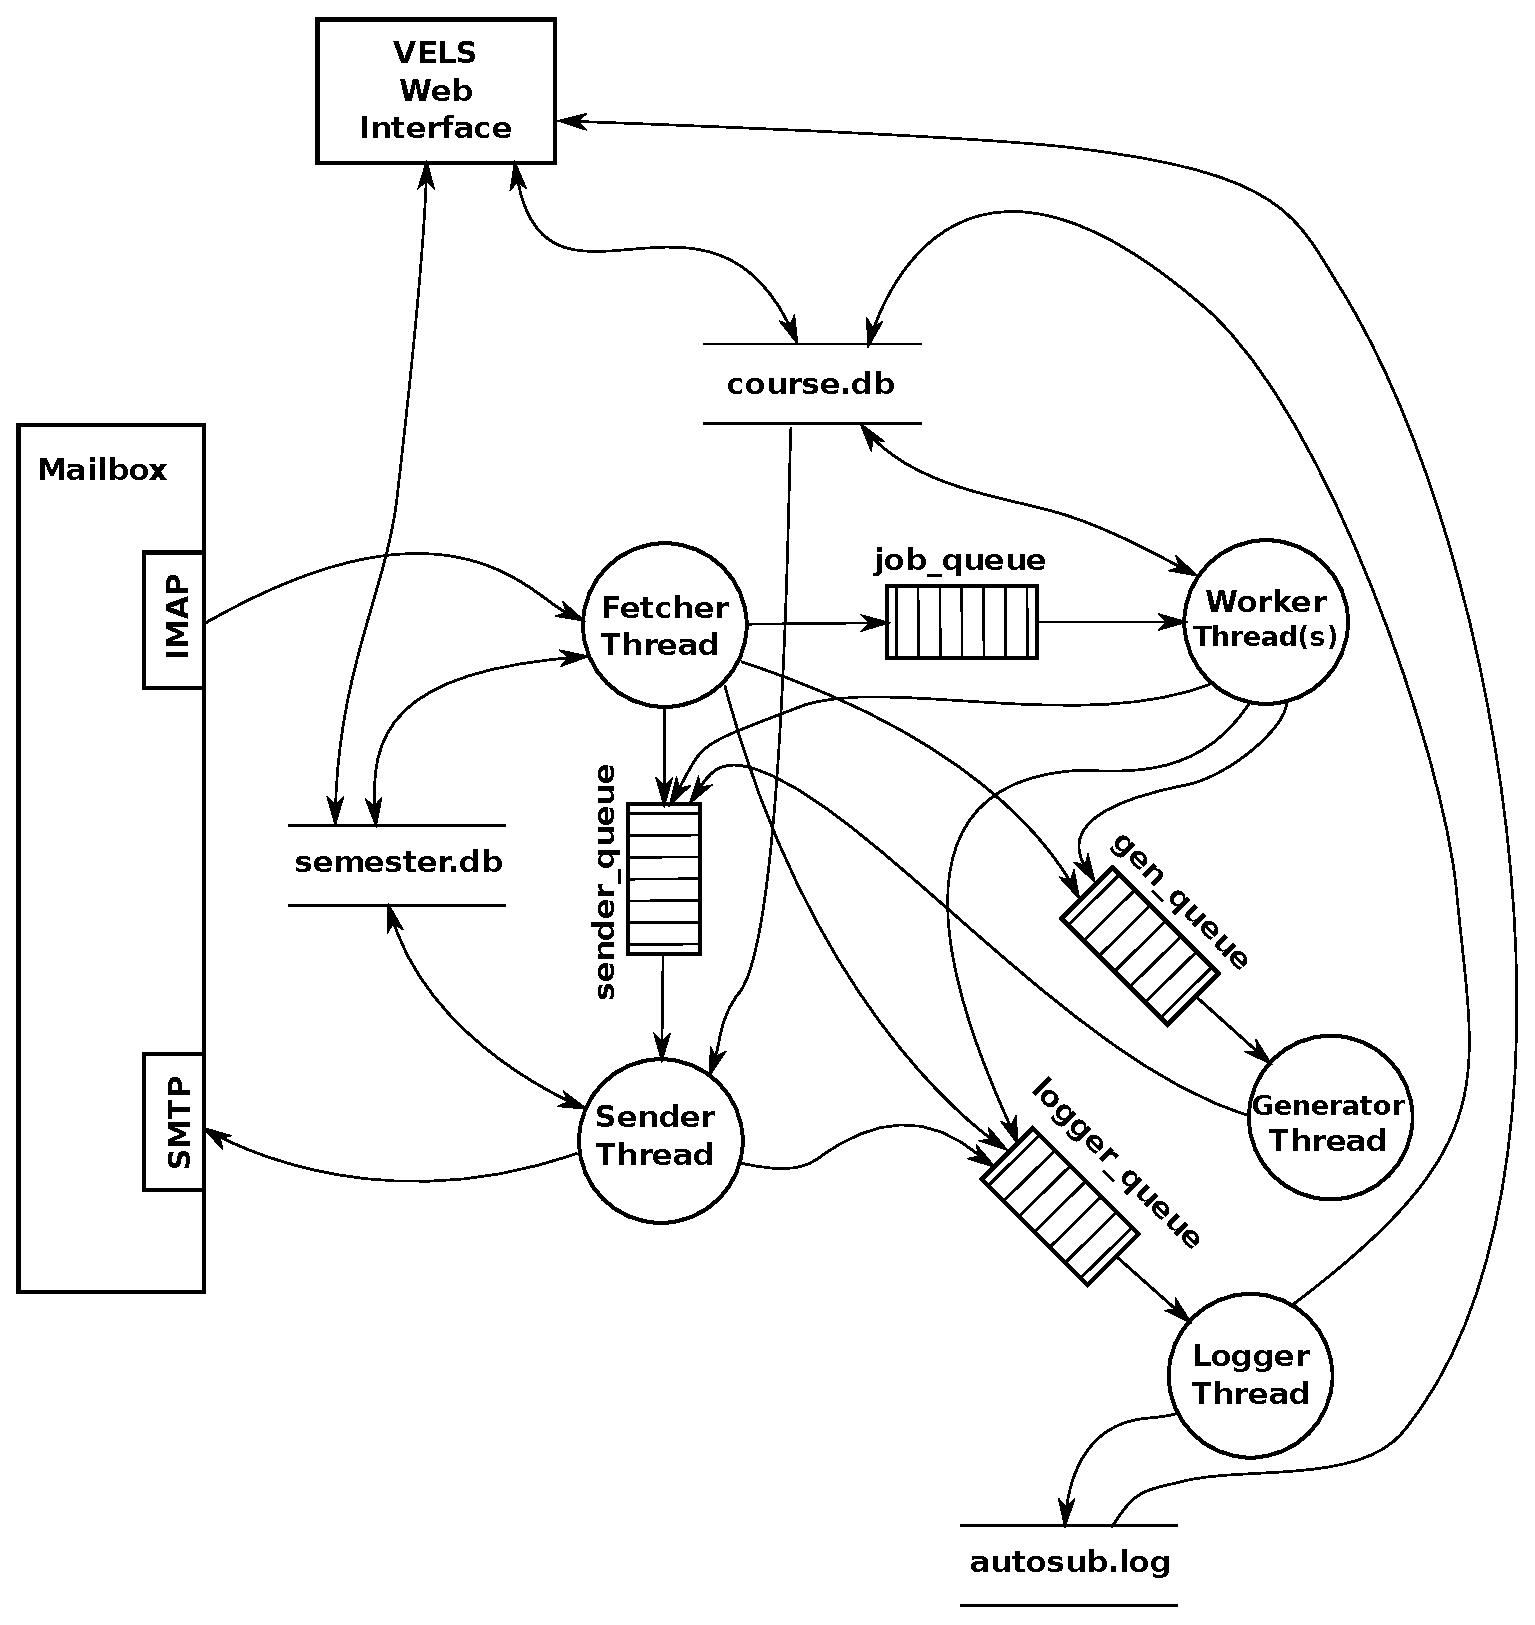
\includegraphics[width=12cm]{images/autosub_future.eps}
    \caption{DFD0 -- High-Level Data-Flows in the Submission System.}
    \label{fig:dfd0}
    \end{center}
\end{figure}


\subsection{Description of Entities}
\begin{description}
    \item [MB] \textbf{Mailbox} \\
    \begin{tabular}{|p{2cm}|p{11cm}|}
        \hline
        Description & Mailbox to interface with students. \\
        \hline
        Rate & Asynchronously by students, once per minute by the E-Learning system. \\
        \hline

        Comment & The Mailbox is used to interface with the students. In depth description of this 
        interface can be found in Section \ref{emailinterface}.
        
        The Mailbox is accessed via \gls{imap} for reading new e-mails and \gls{smtp} to send e-mails.

        After the action triggered by an received e-mail has been processed, the e-mail shall be archived 
        into a configurable folder on the e-mail server.
        \\
        \hline
    \end{tabular}
    \item [1] \textbf{Fetcher Thread} \\
    \begin{tabular}{|p{2cm}|p{11cm}|}
        \hline
        Description &  Fetch E-Mails from the Mailbox.\\
        \hline
        Rate & Periodically once a minute (by default -- period shall be configurable). \\
        \hline

        Comment & The Fetcher Thread periodically checks the Mailbox for new mails. These new
        mails are sorted in the fetcher thread an actions are triggered based on the messages.
        To decide which action is the correct one for a particular e-mail, the user E-mail 
        address and the subject are evaluated. The following use cases are possible.
        \begin{itemize}
        \item New user has to be created.
        \item Task wants to be submitted.
        \item Question wants to be asked.
        \item User status wants to be known.
        \end{itemize}
    
        Further Information concerning the email interface can be be seen in Section \ref{interactions} 
        \\
        \hline
    \end{tabular}
    \newpage
    \item [2] \textbf{Worker Thread(s)} \\
    \begin{tabular}{|p{2cm}|p{11cm}|}
        \hline
        Description & Test the task submissions of students. \\
        \hline
        Rate & Asynchronously triggered upon arrival of a new task submission by a student. \\
        \hline
        Comment & The worker threads are the ones which do the actual work of testing submissions
        by a student. If the Fetcher Thread receives an e-mail with a result submission, a new
        message is added to the job\_queue. The worker threads are using a blocking read on the
        job\_queue to wait for work, as soon as the new message is added by the Fetcher thread one
        of the workers will read it and start the tests for the users submission.
         
        The tests themselves are implemented externally in a bash script. This script is expected
        to return with 0 on success, and 1 if the tests failed. Additional information
        (e.g. error-messages) are expected in a file called {\tt error\_msg} in the  unsuccessful case.
        \\
        \hline
    \end{tabular}

    \item [3] \textbf{Sender Thread} \\
    \begin{tabular}{|p{2cm}|p{11cm}|}
        \hline
        Description & Sends E-mails to the Students \\
        \hline
        Rate & Triggered by Fetcher, Worker or Generator Thread. \\
        \hline

         Comment & If a message has to be returned to the student, the thread that wants to send the
            message just puts the necessary information into the sender\_queue. The sender thread
            then takes that information, formats an e-mail and sends it out using \gls{smtp}.

            The unique message-id is passed from the fetcher (possibly via other threads) to the
            sender thread. If the sender thread has sent out the answering e-mails, the e-mail with
            the given message-id is moved into an archive folder on the mail server.
             \\
        \hline
    \end{tabular}
\newpage
    \item [4] \textbf{Logger Thread}\label{sec:logger} \\
    \begin{tabular}{|p{2cm}|p{11cm}|}
        \hline
        Description & Format log messages and store them in the log file. \\
        \hline
        Rate & Triggered by all other threads. \\
        \hline
         Comment & In order to enforce a common logging format, and allow the setting of a common
            log-level, all threads just put their log-messages into the logger\_queue. The
            logger thread decides (depending on the log-level) whether or not the message shall
            be logged or not. If so, the message is formatted and written to the log file.

            The following log-levels shall be implemented (from lowest to highest):
                \begin{description}
                \item [DEBUG:] Print all kind of information that might be helpful to debug
                    problems. This includes, what user sent which e-mail, what action
                    was taken, what was the result of that action.
                \item [INFO:] Information that might be of interest, even if not in debugging
                    mode.
                \item [WARNING:] A problem occurred, but it did not lead to a long-term problem
                    (e.g. could not connect to the mailserver, but after retrying it worked).
                \item [ERROR:] A problem that lead to a long-term malfunction of the submission
                    system occurred, the system will not be able to recover from this problem.
                \end{description}
        \\
        \hline
    \end{tabular}

    \item [5] \textbf{Generator Thread} \\
    \begin{tabular}{|p{2cm}|p{11cm}|}
        \hline
        Description & Generate a (unique) example for a user. \\
        \hline
        Rate & Triggered by registration of a new user, and successful submission of a task.  \\
        \hline
        Comment & The tasks are tailored for each student using randomized parameters. 

            The generation of a task is done as soon as it is needed e.g. for the first
            task after the user registered, for all the other tasks, as soon as the previous
            task has successfully been submitted.

            The Generator Thread is blocking on the gen\_queue, until the generation of a new
            example is requested. As soon as the example was generated, a request to send it
            out is put into the sender\_queue.
        \\
        \hline
    \end{tabular}
\end{description}

\subsection{Description of Message-Queues}

\begin{description}
\item [job\_queue] The job\_queue is used to trigger worker threads to start testing solutions 
    that were received. The messages in the job\_queue are comprised of the following fields:
    \begin{itemize}
        \item {\bf UserId:} The unique User ID of the user who submitted this solution.
        \item {\bf UserEmail:} The e-mail address of the user who submitted this solution.
        %\item {\bf message_type:} PRESENT IN THE CODE; BUT NOT USED?? THIS IS GOING TO THE WORKER, SO THERE IS ONLY ONE TYPE, REALLY!
        \item {\bf taskNr:} Number of the task that solution has been submitted for.
        \item {\bf MessageId:} The unique message-id of the e-mail on the server.
    \end{itemize}
\item [sender\_queue] If a thread wants to send an e-mail to a user, the sender thread is notified via this queue. 
    The data needed by the sender thread is in the messages in the sender\_queue. These messages consist of the following fields:
    \begin{itemize}
        \item {\bf UserId:} The unique User ID of the user who shall receive this e-mail.
        \item {\bf recipient} E-Mail address of the recipient (the content of the 'To' field in the e-mail).
        \item {\bf message\_type} The message type is used to decide on how to format the e-mail, and 
            whether or not additional e-mails have to be sent out (e.g. when a question is handled). 
            Possible message\_types are:

            \begin{itemize}
            \item {\tt Task} -- A task description.
            \item {\tt Success} -- A Task has been tested successfully.
            \item {\tt Failed} -- An error message for a failed test-run of a result submission.
            \item {\tt SecAlert} -- Scanning the code revealed that this might be an attack on the system.
            \item {\tt TaskAlert} -- An error message for failures in files that were created for tasks.
            \item {\tt InvalidTask} -- A result submission for a non-existent task.
            \item {\tt Usage} -- An e-mail with usage explanation shall be sent to the student. 
            \item {\tt Question} -- Confirm that a question was received.
            \item {\tt QFwd} -- Forward a question to the administrator.
            \item {\tt Welcome} -- Send a welcome message to a new student.
			\item {\tt NotAllowed} -- A user who is not on the whitelist sent a mail to the system.
            \end{itemize}

        \item {\bf Task} Number of the task that message concerns (e.g. the current one if the test failed, 
        the next one if the task description shall be sent).
        \item {\bf MessageId:} The unique message-id of the e-mail on the server.
    \end{itemize}
\item [logger\_queue] Trigger the logger to write a log message about an event that happened.
    \begin{itemize}
        \item {\bf msg:} The text that describes the event that shall be logged.
        \item {\bf type:} The log-level of this log message; available log-levels are DEBUG, INFO, 
            WARNING and ERROR (see specification of Logger Thread in Section \ref{sec:logger} for details).
        \item {\bf loggername:} Name of the thread that reported the event that shall be logged.
    \end{itemize}
\item [gen\_queue] The gen\_queue is used to trigger the Generator Thread to generate a new (variant of) a 
    task. That means that certain parameters of the task are randomized, in order to assure that each student 
    receives his/her very own example. 
	\begin{itemize}
        \item {\bf UserId:} The unique UserID of the User for whom the task is generated.
        \item {\bf UserEmail:} E-Mail address of the User for whom the task is generated.
        \item {\bf TaskNr:} Number of the task that shall be generated.
        \item {\bf MessageId:} The unique message-id of the e-mail on the server.
    \end{itemize}
\end{description}

\subsection{Description of Datastores}

\subsubsection{autosub.log}

The log file shall contain log-messages formatted as follows:

\begin{verbatim}
<date> <time> [<loggername>\t] <log-level:> <log-message>
\end{verbatim}

Some examples for log-messages could look like this:

\begin{verbatim}
2015-06-20 20:36:32,813 [Worker1     ] INFO: Starting Worker1
2015-06-20 20:36:32,813 [Worker2     ] INFO: Starting Worker2
2015-06-20 20:36:32,814 [Worker3     ] INFO: Starting Worker3
...
2015-06-21 08:06:44,526 [fetcher     ] WARNING: Failed to select inbox
...
2015-06-22 16:05:51,255 [fetcher     ] DEBUG: closed connection to imap
server
\end{verbatim}

\subsubsection{.cfg File}
A .cfg file may be passed to the submission system when the daemon is started. If no .cfg file
is specified, the used file is default.cfg. The groups and fields in the config file are as follows:

\begin{tabular}{|p{2.5cm}|p{2.5cm}|p{8cm}|}
\hline
{\bf Group} & {\bf Field} & {\bf Description} \\
\hline
\hline
imapserver & servername & Hostname.domain of the IMAP server.\\
\hline
imapserver & serverport & Port to be used.\\
\hline
imapserver & security & Security protocol to be used when connecting 
    Possible values: none ssl starttls \\
\hline
imapserver & username & Username to be used to login. \\ 
\hline
imapserver & password & Password to be used to login. \\
\hline
imapserver & email & Email address at the IMAP server. \\
\hline
\hline
smtpserver & servername & Hostname.domain of the SMTP server.\\
\hline
smtpserver & serverport & Port to be used. \\
\hline
smtpserver & security & Security protocol to be used when connecting.
    Possible values: none ssl starttls \\
\hline
smtpserver & username & Username to be used to login. \\
\hline
smtpserver & password & Password to be used to login. \\
\hline
smtpserver & email & Email address at the SMTP server. \\
\hline
\hline
general & num\_workers & Number of Worker threads. This influences how many
	tests can conducted in parallel. \\
\hline
general & queue\_size & Size of the thread communication queues. \\
\hline
general & poll\_period & Period in seconds at which the mailbox is checked.\\
\hline
general & course\_name & The name of course.\\
\hline
general & semesterdb & The name and path of the database that shall be used for data specific to
    this semester. (default: semester.db) \\
\hline
general & coursedb & The name and path of the database that shall be used for data specific to
    this course. (default: course.db)\\
\hline
general & logfile & The name and path of the autosub logfile. (default: autosub.log)\\
\hline
general & auto\_advance & Decides if users get auto advanced to a task which is
    activated by its TaskStart. Possible values: yes no (default:no) \\
\hline
challenge & num\_tasks & The mode in which to run (exam or normal).\\
\hline
challenge & mode & The mode in which to run (exam or normal). \\ 
\hline
\end{tabular}

\newpage

\subsubsection{semester.db}

The semester database is used to store all data that is specific to one semester. This includes,
users, parametrization of tasks assigned for users, statistics, etc. .

The database semester.db contains the following tables (and entries in those tables):

\begin{tabular}{|p{3cm}|p{10cm}|}
\hline
Table Name & Users \\
\hline
Description & Used to collect all necessary information on the Students.\\
\hline
Table Entries & \begin{itemize}
        \item {\bf UserId}: A unique UserID given at registration time (when the first e-mail
            is received from the users e-mail address).
        \item {\bf Name}: The name of the user as specified in the "from" field of the e-mail.
        \item {\bf Email}: The e-mail address of the user as specified in the "from" field of the
            e-mail.
        \item {\bf FirstMail}: Timestamp of the first e-mail received by this user.
        \item {\bf LastDone}: Timestamp of the email that contained the successful solution of the
            last task (only if this user has already finished the last task).
        \item {\bf CurrentTask}: The task the user is currently working on.
        \end{itemize} \\
\hline
\end{tabular}

\begin{tabular}{|p{3cm}|p{10cm}|}
\hline
Table Name & TaskStats \\
\hline
Description & Contains one entry for each available task, collecting statistics on the individual tasks.\\
\hline
Table Entries & \begin{itemize}
        \item {\bf TaskId}: Unique ID of the task.
        \item {\bf NrSubmissions}: Number of solutions received for the task with this TaskId.
        \item {\bf NrSuccessful}: Number of correct solutions received for the task with this TaskId.
        \end{itemize} \\
\hline
\end{tabular}

\begin{tabular}{|p{3cm}|p{10cm}|}
\hline
Table Name & TaskCounters \\
\hline
Description & Implements counters for certain events, examples for such events are: e-mail received, e-mail sent, 
question received, new user.\\
\hline
Table Entries & \begin{itemize}
        \item {\bf CounterId}: Unique ID of the counter.
        \item {\bf Name}: Name of the counter.
        \item {\bf Value}: Value of the counter.
        \end{itemize} \\
\hline
\end{tabular}

\begin{tabular}{|p{3cm}|p{10cm}|}
\hline
Table Name & UserTasks \\
\hline
Description & Used to map configured tasks to users -- e.g. store the generated examples so they can be 
    fetched later on for testing.\\
\hline
Table Entries & \begin{itemize}
    \item {\bf TaskNr}: Unique number of the task.
    \item {\bf UserId}: Unique ID of the user -- the combination of TaskNr and UserId make the entry unique.
    \item {\bf TaskParameters}: Either the parameters that describe the setting for this particular student, or a value that can be
        used to derive the parameters from.
    \item {\bf TaskDescription}: Message that describes the task that was specifically generated for the student.
        and shall be sent to the student.
    \item {\bf TaskAttachments}: List of attachments that shall be sent to the student (path+filename).
    \item {\bf NrSubmissions}: Number of submissions the student has done for this task.
    \item {\bf FirstSuccessful}: Number of the first successful submission.
\end{itemize} \\
\hline
\end{tabular}



\begin{tabular}{|p{3cm}|p{10cm}|}
\hline
Table Name & UserWhiteList \\
\hline
Description & A Whitelist of E-Mail addresses that shall be authorized to interact with the system.\\
\hline
Table Entries & \begin{itemize}
        \item {\bf UniqueId}: Unique ID in the whitelist table.
        \item {\bf Email}: E-mail address that shall be authorized to interact with the system.
        \end{itemize} \\
\hline
\end{tabular}

\subsubsection{course.db}

In contrast to semester.db, course.db consists configuration data that will very likely be reused in the next
semester. This seperation makes it very easy to start a new semester: just backup semester.db to some safe
location and remove it in the original location (a new empty one will be made automatically). 

Then use the VELS web interface to perform the small modifcations (year/semester, deadlines, etc.) needed in course.db.

\begin{tabular}{|p{3cm}|p{10cm}|}
\hline
Table Name & SpecialMessages \\
\hline
Description & A collection of texts that shall be sent, in the case special events. \\
\hline
Table Entries & \begin{itemize}
    \item {\bf EventName}: Currently the following events are implemented:
        \begin{itemize}
        \item WELCOME -- A welcome message that is sent upon first e-mail from a student and
                that gives an explanation of how the system works.
        \item USAGE -- In case an e-mail that can not be interpreted is received, this message
                shall be sent to the user.
        \item QUESTION -- A message that is sent as a confirmation if a question was received.
        \item INVALID -- A message that is sent, in case a result for an invalid task has
                been received.
        \item CONGRATS -- A message that congratulates the student upon solving the last task.
        \item REGOVER -- A message sent in case a student tries to register after the registration 
                deadline has passed.
        \item NOTALLOWED -- A mesage sent in case the student is not on the whitelist.
        \item CURLAST -- A mesage sent to inform the student that he has solved the current last task.
        \item DEADTASK -- A mesage sent to inform the student that he submitted a task which's deadline is allready over.
            \end{itemize}
        \item {\bf Text}: The text that shall be sent in case of the event {\bf EventName} occurs.
        \end{itemize} \\
\hline
\end{tabular}

\begin{tabular}{|p{3cm}|p{10cm}|}
\hline
Table Name & TaskConfiguration \\
\hline
Description & Used to configure tasks, including their order, the scripts used to test submissions, etc.\\
\hline
Table Entries & \begin{itemize}
    \item {\bf TaskNr}: The unique number of the task -- this number is used to establish the order 
        of tasks as received by the students.
    \item {\bf TaskStart}: Timestamp of when the task shall be available for students (if any). 
    \item {\bf TaskDeadline}: The deadline until which the task has to be successfully submitted (if any).
    \item {\bf PathToTask}: The root directory of the task (so it does not have to be specified for all 
        the entries).
    \item {\bf GeneratorExecutable}: The executable (script, binary, etc.) used to generate unique examples 
        for each student. If this is not set, all students will receive the same task.
    \item {\bf TestExecutable}: The executable (script, binary, etc.) used to test the results submitted
        by the students.
    \item {\bf Score:} The points the student scores by solving this task.
    \item {\bf TaskOperator:} The e-mail address of the course operator, who is responsible for this task.
    \end{itemize}
    
\\
\hline
\end{tabular}

\begin{tabular}{|p{3cm}|p{10cm}|}
\hline
Table Name & GeneralConfig \\
\hline
Description & Store some general configuration for the semester.\\
\hline
Table Entries & \begin{itemize}
    \item {\bf ConfigItem}: Name of the Configuration Item.
        The following configuration items are available:
        \begin{itemize}
        \item {\tt registration\_deadline} -- the deadline for students to register.
        \item {\tt num\_tasks} -- the number of tasks available in this semester.
        \item {\tt archive\_dir} -- the name of the directory on the mail-sever into
            which the answered messages shall be moved.
        \item {\tt admin\_email} -- the email of the admin for the course.
        \item {\tt challenge\_mode} -- the mode for the course : normal or exam.
        \end{itemize}
    \item {\bf Content}: Content of the Configuration Item.
    \end{itemize} \\
\hline
\end{tabular}
